\documentclass[handout]{beamer}
%\documentclass[presentation]{beamer}
\usepackage[utf8]{inputenc}
\usepackage{amsmath, pdfpages, pdflscape, lscape, color, listings, hyperref, amssymb, graphicx,textcomp,varioref, afterpage, subcaption, float, bm, tikz}

\global
\newcommand{\Fig}[1]{Figure \ref{#1}}
\newcommand{\fig}[1]{figure \ref{#1}}
\newcommand{\tab}[1]{table \ref{#1}}
\newcommand{\eq}[1]{equation \ref{#1}}
\newcommand{\Eq}[1]{Equation \ref{#1}}
\newcommand{\alg}[1]{algorithm \ref{#1}}
\newcommand{\Alg}[1]{Algorithm \ref{#1}}
\newcommand{\chp}[1]{chapter  \ref{#1}}
\newcommand{\Chp}[1]{Chapter  \ref{#1}}
\newcommand{\e}[1]{\cdot 10^{#1}}
\newcommand{\h}{\hbar}
\newcommand{\der}[2]{\frac{\partial #1}{\partial #2}}
\newcommand{\dder}[2]{\frac{\partial^2 #1}{\partial #2^2}}
\newcommand{\p}{\boldsymbol{P}}
\newcommand{\q}{\boldsymbol{q}}
\newcommand{\norm}[1]{\left\lVert#1\right\rVert_{\!Q}}
\newcommand{\inner}[1]{\left\langle#1\right\rangle_{\!Q}}
\newcommand{\coef}[2]{\frac{\inner{#1,#2}}{\norm{#2}^2}}

\newcommand{\gooditem}[1]{\setbeamercolor{item}{fg=green}\item #1}
\newcommand{\baditem}[1]{\setbeamercolor{item}{fg=red}\item #1}

\DeclareMathOperator*{\argmin}{argmin}
\DeclareMathOperator*{\argmax}{argmax}

\newcommand{\E}[1]{\mbox{E}\!\left(#1\right)}
\newcommand{\Var}[1]{\mbox{Var}\!\left(#1\right)}
\newcommand{\Cov}[1]{\mbox{Cov}\!\left(#1\right)}



\setbeamertemplate{blocks}[rounded][shadow=false]


\usefonttheme[onlysmall]{structurebold}
% Use a bold face title font
\setbeamerfont{title}{series=\bfseries}
\setbeamerfont{frametitle}{series=\bfseries}

% This is not created yet, but should be...
%\usecolortheme{simula}

% Suppress navigation symbols
\setbeamertemplate{navigation symbols}{}

\definecolor{listingsstringcolor}{rgb}{0,0.5,0}
\definecolor{listingskeywordcolor}{rgb}{0,0,1}
\definecolor{listingsbasiccolor}{rgb}{0.0,0.0,0.0}

\definecolor{myred}{RGB}{190,0,0}

 \newcommand{\listingsfont}{\sffamily}

 \lstset{
    language=python,
     basicstyle=\color{listingsbasiccolor},
    keywordstyle=\color{listingskeywordcolor},
    stringstyle=\color{listingsstringcolor},
 tabsize=4,                       % sets default tabsize to 2 spaces
 morekeywords={as, assert, with, yield},
escapeinside={||},
basicstyle=\ttfamily\footnotesize,
columns=fixed
}

\newenvironment{chaospy}[1]
{\color{gray!30!black}
     \usebackgroundtemplate{
   \begin{tikzpicture}[remember picture, overlay]
     \node[anchor = center, opacity=.15] (image) at (current page.center) {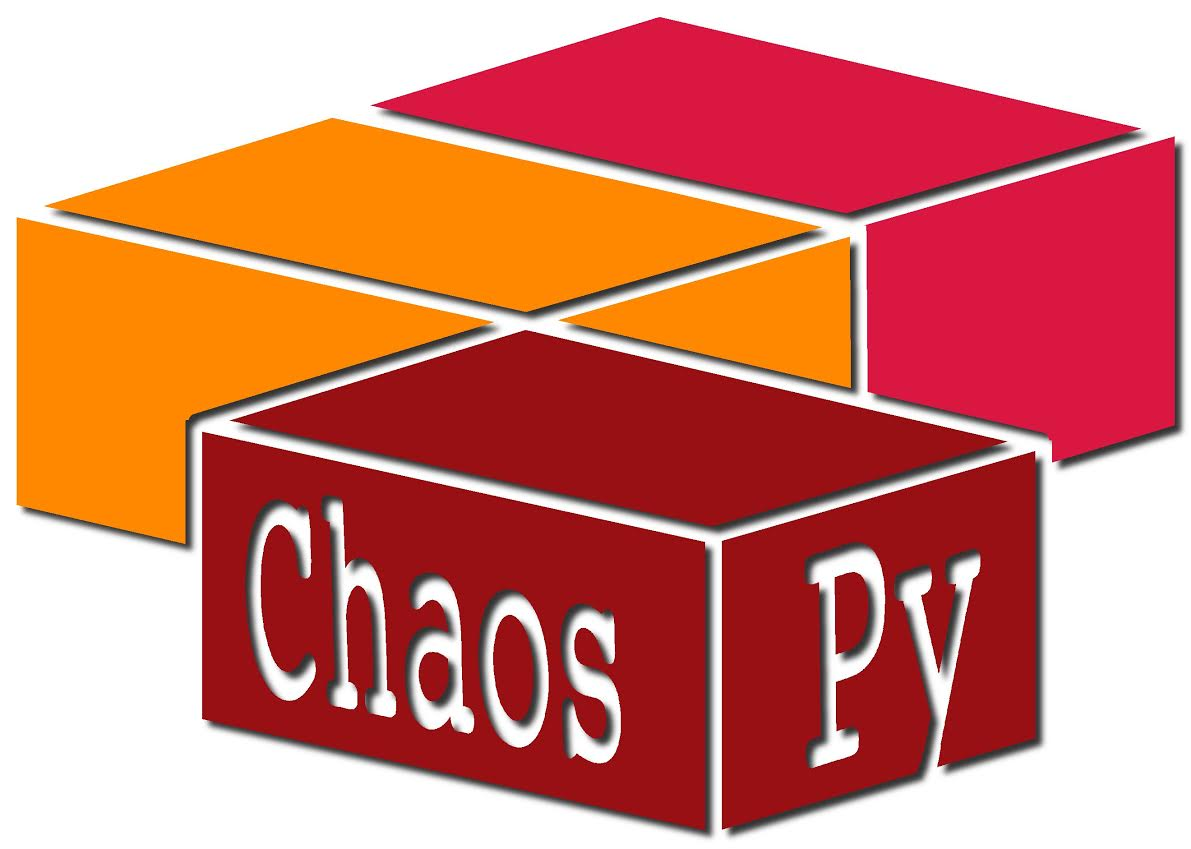
\includegraphics[scale=0.25]{chaospy_logo.jpg}};
   \end{tikzpicture}}
     \begin{frame}[fragile, environment=chaospy]
    \frametitle{{#1}}}
{\end{frame}}


\definecolor{keywords}{RGB}{255,0,90}
\definecolor{comments}{RGB}{0,0,113}
\definecolor{red}{RGB}{160,0,0}
\definecolor{green}{RGB}{0,150,0}


\setbeamercolor{title}{fg=myred}
\setbeamercolor{frametitle}{fg=black!65!white,bg=white}
\setbeamercolor{normal text}{fg=black!75!white,bg=white}
\setbeamercolor{structure}{fg=black,bg=white}



\graphicspath{{./figures/}}


\title{Chaospy: \\ A modular implementation of polynomial chaos expansions and Monte Carlo methods}
\author{Simen Tennøe}
\institute{University of Oslo, CINPLA}

\begin{document}


\begin{frame}
  \maketitle
\end{frame}


% \begin{frame}[fragile]{Chaospy is a Python toolbox for uncertainty quantification, developed by Jonathan Feinberg}
%   \begin{center}
%      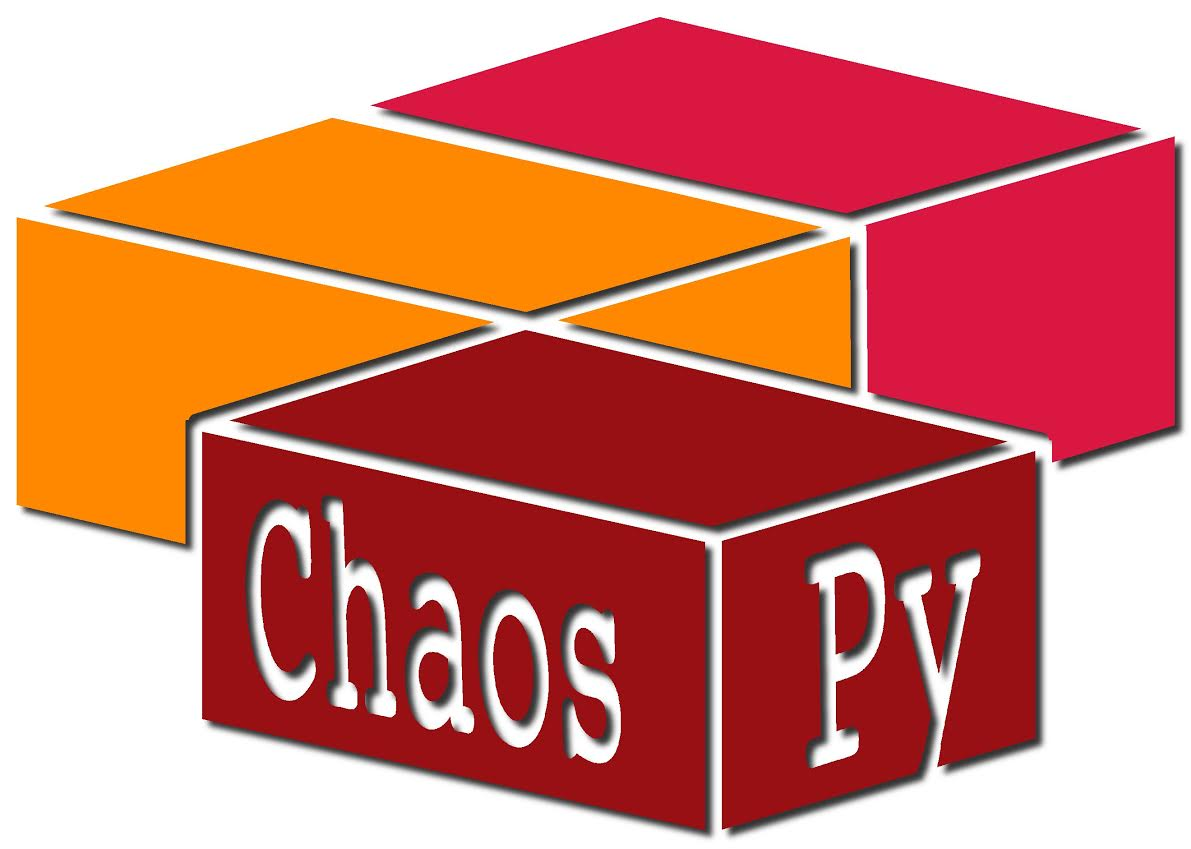
\includegraphics[width=.8\textwidth]{chaospy_logo.jpg}
%   \end{center}
% %     \begin{alert}{A very basic introduction to scientific Python programming:}
% %     \scriptsize
% %       \href{http://hplgit.github.io/bumpy/doc/pub/sphinx-basics/index.html}{http://hplgit.github.io/bumpy/doc/pub/sphinx-basics/index.html}\\
% % %\verb;http://hplgit.github.io/bumpy/doc/pub/sphinx-basics/index.html;
% % %   \end{alert}
% %   \begin{alert}{Installation instructions:}\\
% %   \scriptsize
% %       \href{https://github.com/hplgit/chaospy}{https://github.com/hplgit/chaospy}\\
% % %\verb;http://github.com/hplgit/chaospy/;
% %   \end{alert}
% \end{frame}



\begin{frame}[fragile]{This presentation focuses on Chaospy, a Python toolbox for uncertainty quantification}




  \begin{tikzpicture}[remember picture, overlay, font=\sffamily]
  \node [align=left, xshift=-0.4\textwidth,yshift=0.1\textwidth] (image1) at (current page.center)
      {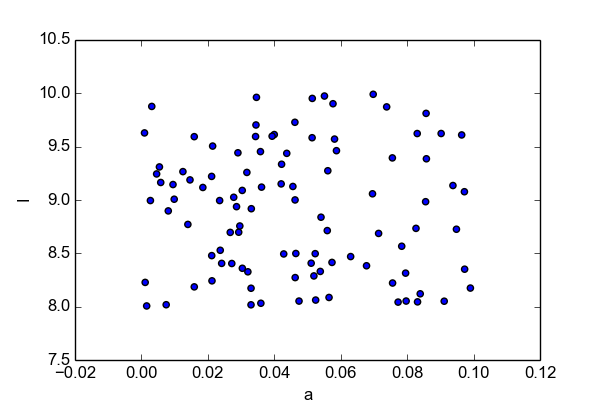
\includegraphics[width = 0.25\textwidth]{samples.png}};
  \node[align=left] at (image1.east) {\hspace{4.5cm} \bf Monte Carlo methods};
  \end{tikzpicture}

\pause


    \begin{tikzpicture}[remember picture, overlay, font=\sffamily]
      \node [align=left, xshift=-0.2\textwidth,yshift=-0.1\textwidth] (image2) at (current page.center)
            {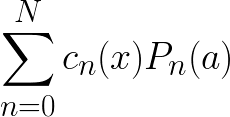
\includegraphics[width = 0.25\textwidth]{pc.png}};
      \node[align=left] at (image2.east) {\hspace{4cm} \bf Polynomial Chaos};
    \end{tikzpicture}


    \pause

      \begin{tikzpicture}[remember picture, overlay, font=\sffamily]
        \node [align=left, xshift=0\textwidth,yshift=-0.3\textwidth] (image3) at (current page.center)
              {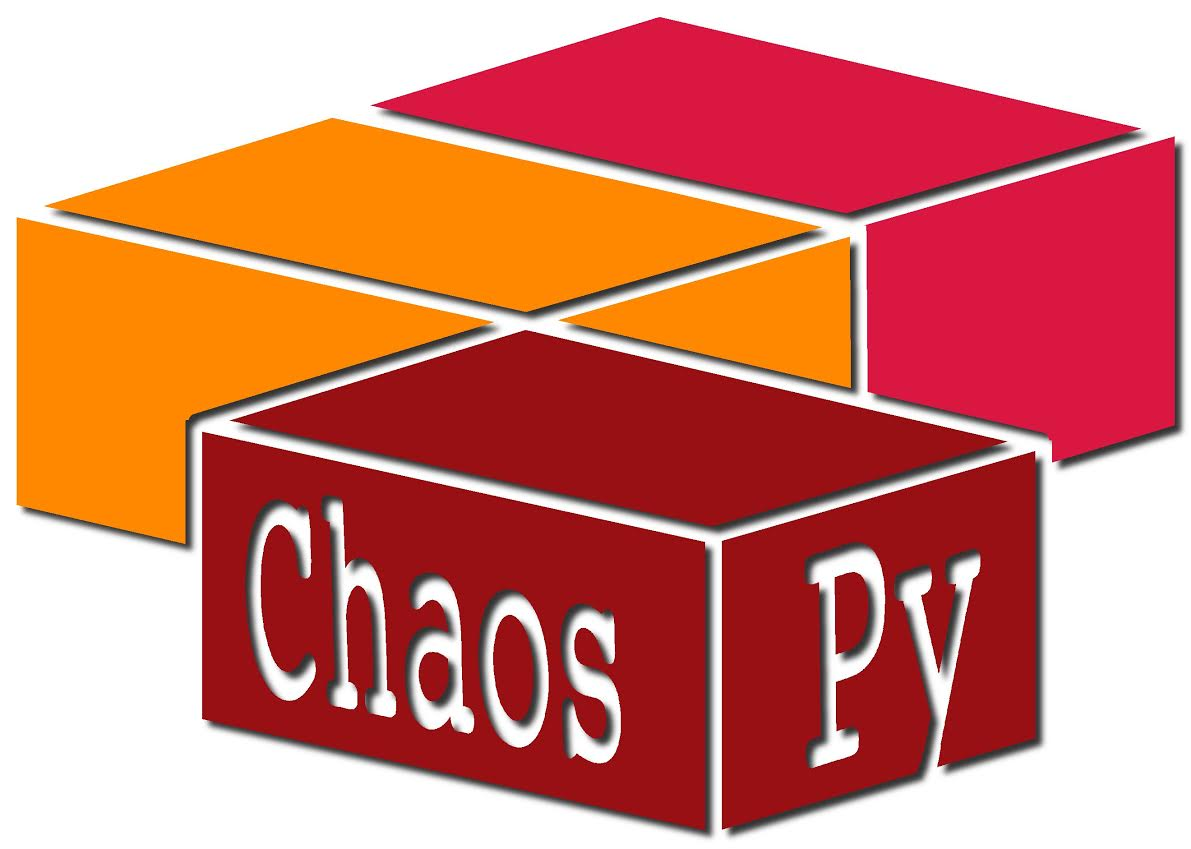
\includegraphics[width = 0.2\textwidth]{chaospy_logo.jpg}};
        \node[align=left] at (image3.east) {\hspace{5cm} \bf Properties of Chaospy};
      \end{tikzpicture}


\end{frame}



 \begin{frame}
 \frametitle{Chaospy is a Python toolbox for uncertainty quantification}

%\vspace{-5mm}
 Chaospy implements advanced Monte Carlo methods and Polynomial Chaos expansions.

 \begin{columns}
      \column{.5\textwidth}
      \begin{center}
                 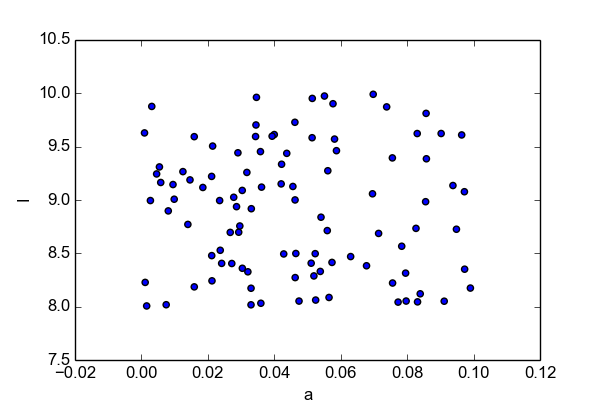
\includegraphics[width=0.5\textwidth]{samples.png}
      \end{center}
      \column{.5\textwidth}
      \begin{center}
                   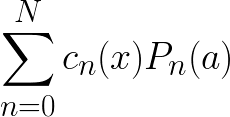
\includegraphics[width=0.5\textwidth]{pc.png}
      \end{center}
  \end{columns}

  \vspace{5mm}
\pause
Chaospy is modular with a programming syntax that lies close the the mathematical theory.

\begin{columns}
     \column{.5\textwidth}
     \begin{center}
                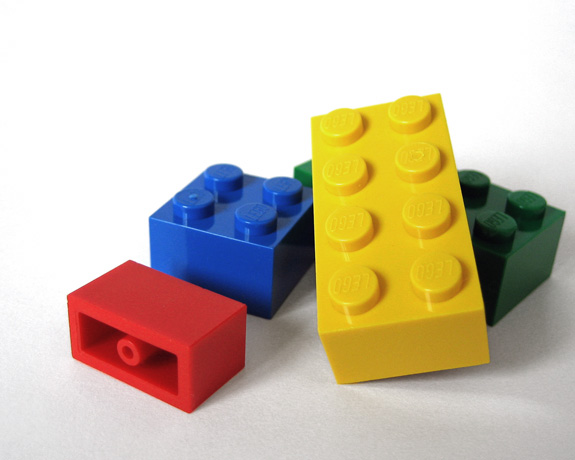
\includegraphics[width=0.5\textwidth]{lego.jpg}
     \end{center}
     \column{.5\textwidth}
     \begin{center}

  \lstinline|dist = chaospy.Uniform(0, 0.1)|

    \end{center}

 \end{columns}

 \end{frame}


% \begin{frame}
%  \frametitle{Chaospy implements advanced Monte Carlo methods and Polynomial Chaos expansions.}
%
%  \begin{columns}
%       \column{.5\textwidth}
%       \begin{center}
%                  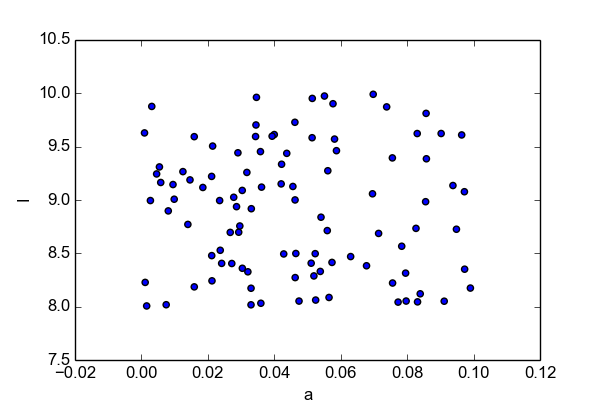
\includegraphics[width=1\textwidth]{samples.png}
%       \end{center}
%       \column{.5\textwidth}
%       \begin{center}
%                    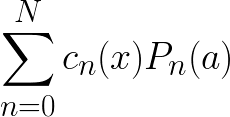
\includegraphics[width=1\textwidth]{pc.png}
%       \end{center}
%   \end{columns}
%
%  \end{frame}
%
%
% \begin{frame}
%   \frametitle{Chaospy is modular with a syntax that lies close the the mathematical theory.}
%
%   \begin{columns}
%        \column{.5\textwidth}
%        \begin{center}
%                   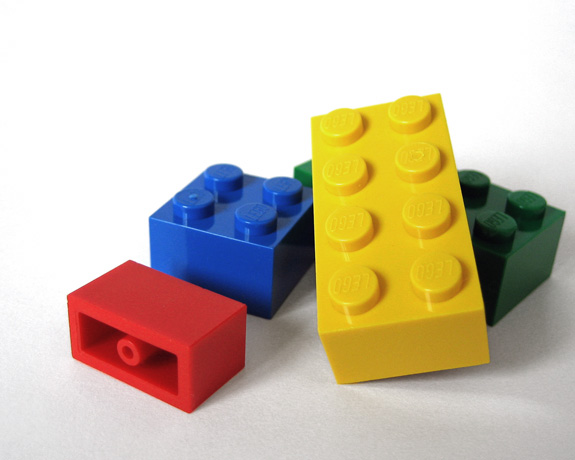
\includegraphics[width=1\textwidth]{lego.jpg}
%        \end{center}
%        \column{.5\textwidth}
%        \begin{center}
%
%     \lstinline|dist = chaospy.Uniform(0, 0.1)|
%
%       \end{center}
%
%    \end{columns}
% \end{frame}




% \begin{frame}{Transformations can be used to model dependent
%     variables effectively as a parameterization of independent
%     variables}{}
%     \begin{align*}
%         \hat u_M(x; q)
%         \onslide<2->{= \hat u_M(x; T(r))}
%         \onslide<3->{= \sum_{n=0}^N c_n(x) P_n(r)}
%     \end{align*}
% \end{frame}





\begin{frame}
 \frametitle{Our model problem will be a simple differential equation}
 \vspace{-10mm}
  \begin{align*}
    \frac{d u(x)}{dx} & =-au(x),\qquad u(0) = I
  \end{align*}
  \vspace{-5 mm}
  \begin{itemize}
    \item[$u$] The quantity of interest
    \item[$x$] Spatial location
    \item[$a,I$] Parameters containing uncertainties
  \end{itemize}

\vspace{-5 mm}
 \pause
%Initially assume model parameters:
\begin{align*}
a &\sim \text{Uniform(0, 0.1)} & I& \sim \text{Uniform(8, 10)}
\end{align*}
\pause
\vspace{5 mm}
Analytical solution
\[u(x; a, I) = Ie^{-ax}\]

\pause
\vspace{5mm}
We want to compute E(u) and Var(u).

\end{frame}



%
% \begin{frame}[fragile]
%   {Introducing a testcase as a working example}
%   \pause
%   \begin{align*}
%     \frac{d u(x)}{dx} & =-au(x) & u(0) &= I
%   \end{align*}
%   \begin{itemize}
%     \item[$u$] The quantity of interest
%     \item[$x$] Spatial location
%     \item[$a,I$] Parameters containting uncertainties
%   \end{itemize}
%   \pause
%   \begin{center}
%     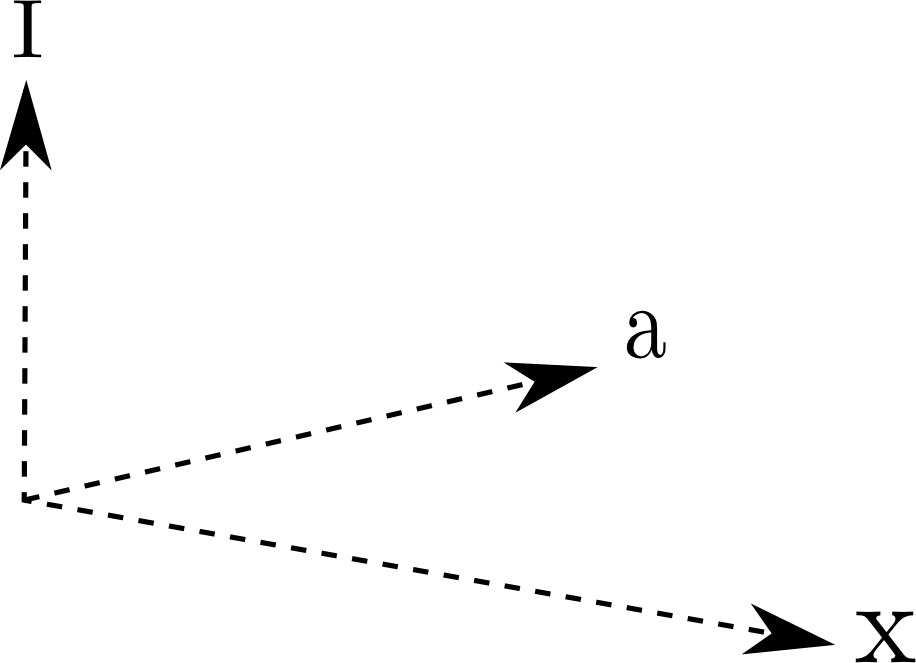
\includegraphics[width=.5\textwidth]{probspace.png}
%   \end{center}
% \end{frame}
%
% \begin{frame}
%  \frametitle{Our model problem will be a simple differential equation}
%  \vspace{-3 mm}
%   \begin{align*}
%     \frac{d u(x)}{dx} & =-au(x), & u(0) &= I
%   \end{align*}
%   \vspace{-2 mm}
%
%   \begin{itemize}
%     \item[$u$] The quantity of interest
%     \item[$x$] Spatial location
%     \item[$a,I$] Parameters containting uncertainties
%   \end{itemize}
% \vspace{5 mm}
%  \pause
%  Initially assume model parameters:
% \begin{align*}
% a &\sim \text{Uniform(0, 0.1)} \sim f_a(a) & I&=1\hbox{ (known)}
% \end{align*}
% \pause
% \vspace{3mm}
% We want to compute E(u) and Var(u).
%
% \end{frame}


%
% \begin{frame}
%  {This model can be analysed analytically}
%
%  Analytical solution
%  \[
%  u(x; a, I) = Ie^{-ax}
%  \]
%
% \pause
% Mean and Variance
%   \begin{align*}
%       \E{u} &=  \int\limits_{-\infty}^{\infty} u(x;a)f_a(a)da=
%             10\int_0^{0.1}e^{-ax}da
%     = 10\frac{1-   e^{-0.1x}}{x} \\
%     \onslide<4->{ \Var{u} & =\int\limits_{-\infty}^{\infty} (u(x;a)-
%     \E{u})^2f_a(a)da \\
%       &= 20\frac{1 - e^{-0.2ax}}{x} - \left(10\frac{1-e^{-0.1x}}{x}\right)^2}
%  \end{align*}
% \end{frame}

%
% \begin{frame}
%  {This model has a analytical solution to compare to our numerical solution}
%
%  Analytical solution:
%  \[
%  u(x; a, I) = Ie^{-ax}
%  \]
% \pause
%
% The errors in our numerical methods are:
%
% \begin{align*}
%     \varepsilon_E &= \int|\E{u} - \E{\hat{u}}|\,dx \\
%     \varepsilon_{Var} &= \int|\Var{u} - \Var{\hat{u}}|\,dx
% \end{align*}
%
%
% \end{frame}




\begin{frame}[fragile]
{In general, models can be analysed using Monte Carlo integration}

    \begin{figure}
    
\includegraphics[width=\textwidth]{MC.png}
  \end{figure}
\end{frame}

%
% \begin{chaospy}{Creating multivariate probability distributions in Chaospy}
% \begin{lstlisting}[language=python]
% dist_a = cp.Uniform(0, 0.1)
% dist_I = cp.Uniform(8, 10)
% |\pause|
% dist = cp.J(dist_a, dist_I)
% \end{lstlisting}
% \end{chaospy}


\begin{chaospy}{Monte Carlo with Chaospy}
    \scriptsize
\begin{lstlisting}[language=python]
import chaospy as cp
import numpy as np

def u(x, a, I):
    return I*np.exp(-a*x)

|\pause|
dist_a = cp.Uniform(0, 0.1)
dist_I = cp.Uniform(8, 10)
dist = cp.J(dist_a, dist_I)
|\pause|
samples = dist.sample(size=1000)
|\pause|
x = np.linspace(0, 10, 100)
|\pause|
samples_u = [u(x, a, I) for a, I in samples]
|\pause|
E = np.mean(samples_u, 0)
Var = np.var(samples_u, 0)
\end{lstlisting}
\end{chaospy}


\begin{frame}
  \frametitle{Convergence of Monte Carlo is slow}
  % \begin{align*}
  %     \varepsilon_E &= \int_0^{10}|\E{u} - \E{\hat{u}}|\,dx &
  %     \varepsilon_{Var} &= \int_0^{10}|\Var{u} - \Var{\hat{u}}|\,dx
  % \end{align*}
  \begin{center}
    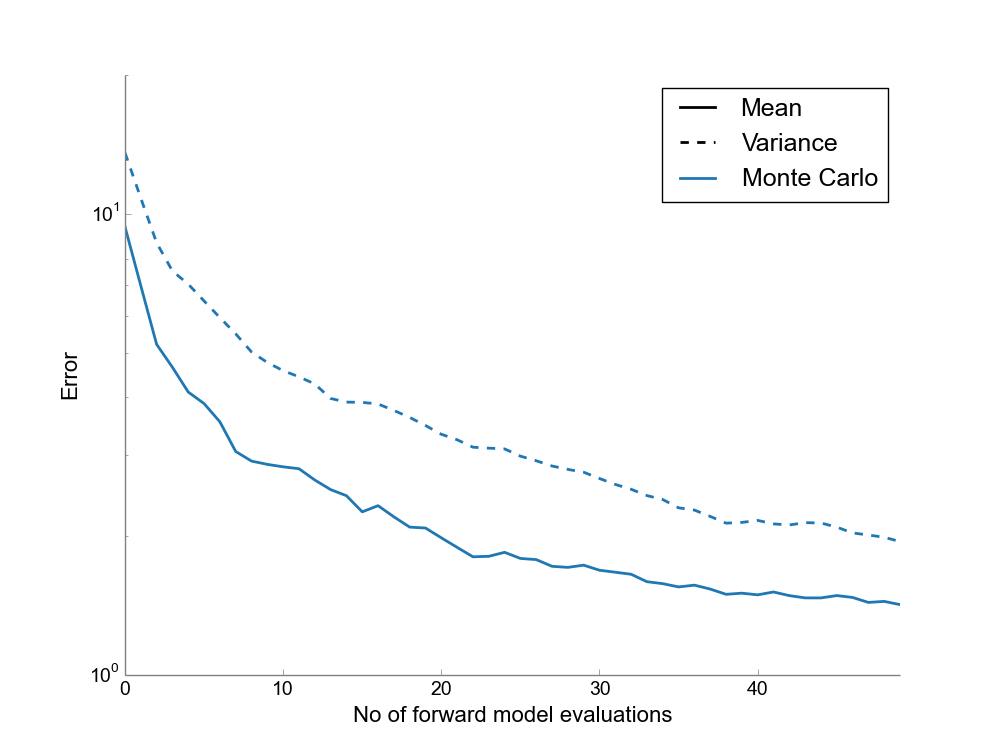
\includegraphics[width=1\textwidth]{MC_convergence_2D.png}
  \end{center}
\end{frame}


% \begin{frame}{Sampling schemes in Chaospy}
% \begin{center}
% {
%     \def\arraystretch{1.2}
%   \begin{tabular}{llll}
%    Key & & &  Name            \\\hline
%      K & & &  Korobov            \\
%      R & & &  (Pseudo-)Random   \\
%      L & & &  Latin hypercube    \\
%      S & & &  Sobol              \\
%      H & & &  Halton             \\
%      M & & &  Hammersley        \\\hline
%      C & & &  Clenshaw Curtis   \\
%      G & & &  Gaussian quadrature\\
%      E & & &  Gauss-Legendre\\\hline
%   \end{tabular}
% }
% \end{center}
%
% \end{frame}



% \begin{frame}{Chaospy have several variance reduction technices used when sampling a distribution}
% \begin{center}{
% \def\arraystretch{1.2}
%   \begin{tabular}{llll}
%    Key & & &  Name            \\\hline
%      R & & &  (Pseudo-)Random   \\\hline
%      \pause
%      K & & &  Korobov            \\
%      L & & &  Latin hypercube    \\
%      S & & &  Sobol              \\
%      H & & &  Halton             \\
%      M & & &  Hammersley        \\\hline
%   \end{tabular}
% }
% \end{center}
% \pause
% In addition Chaospy has support for Antithetic variables.
%
% \end{frame}


\begin{frame}[fragile]
 \frametitle{Chaospy have several variance reduction technices used when sampling a distribution}
 % TODO
 % compare 4 schemes: ' ', 'M', 'S', 'L'
 % remove margins
 \vspace{-2mm}
 \begin{columns}
     \column{.5\textwidth}
     \begin{center}
                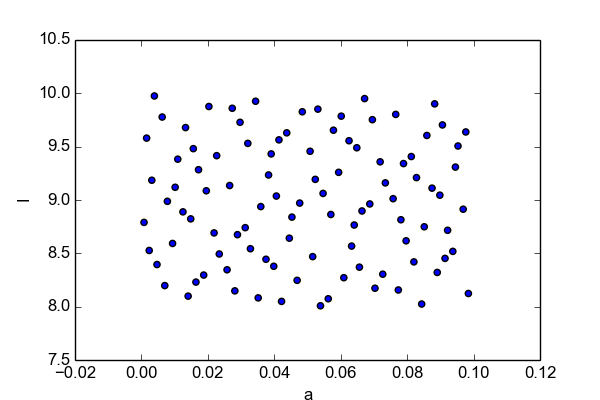
\includegraphics[width=0.65\textwidth]{samples_H.png}

                Hammersley sampling:

                \scriptsize
                \verb;nodes = dist.sample(100, "M");
                \normalsize

                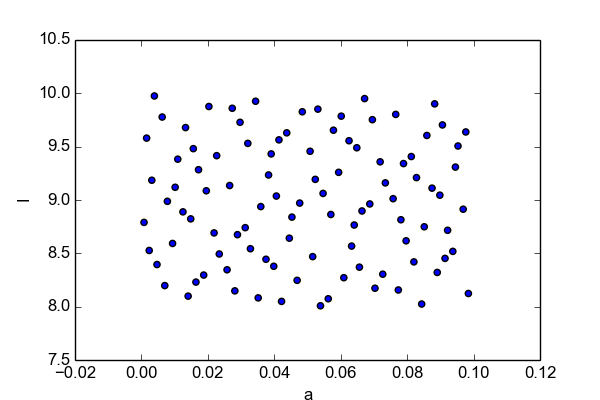
\includegraphics[width=0.65\textwidth]{samples_H.png}

                Halton sampling

                \scriptsize
                \verb;nodes = dist.sample(100, "H");
                \normalsize

     \end{center}
     \column{.5\textwidth}
     \begin{center}
                  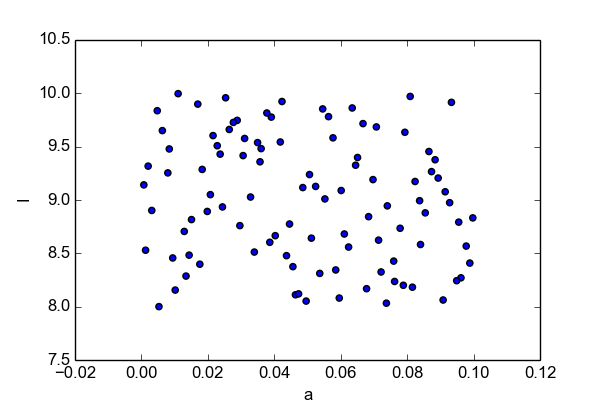
\includegraphics[width=0.65\textwidth]{samples_L.png}

                Latin Hypercube sampling:

                \scriptsize
                \verb;nodes = dist.sample(100, "L");
                \normalsize



                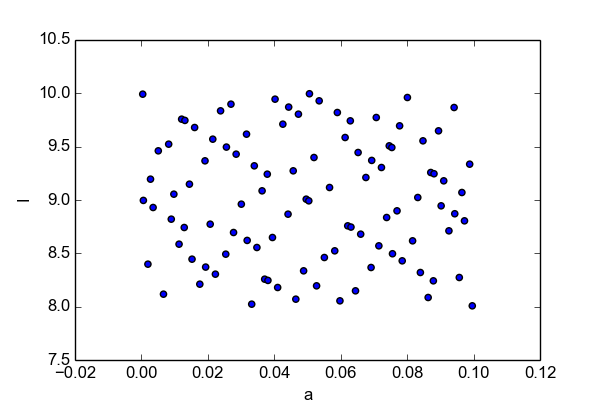
\includegraphics[width=0.65\textwidth]{samples_S.png}

                Sobol sampling

                \scriptsize
                \verb;nodes = dist.sample(100, "S");
                \normalsize
     \end{center}
 \end{columns}
\end{frame}



\begin{chaospy}{Quasi-Monte Carlo with Latin Hypercube sampling}
    \scriptsize
\begin{lstlisting}[language=python]
import chaospy as cp
import numpy as np

def u(x, a, I):
    return I*np.exp(-a*x)


dist_a = cp.Uniform(0, 0.1)
dist_I = cp.Uniform(8, 10)
dist = cp.J(dist_a, dist_I)

samples = dist.sample(size=1000, |\color{red}{rule="L"}|)
|\pause|
x = np.linspace(0, 10, 100)

samples_u = [u(x, a, I) for a, I in samples]

E = np.mean(samples_u, 0)
Var = np.var(samples_u, 0)
\end{lstlisting}
\end{chaospy}


% \begin{frame}
%   \frametitle{Convergence of Monte Carlo is slow}
%   \begin{align*}
%       \varepsilon_E &= \int_0^{10}|\E{u} - \E{\hat{u}}|\,dx &
%       \varepsilon_{Var} &= \int_0^{10}|\Var{u} - \Var{\hat{u}}|\,dx
%   \end{align*}
%   \begin{center}
%     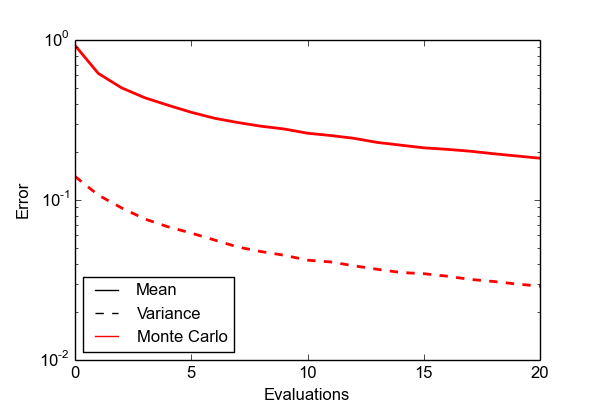
\includegraphics[width=0.75\textwidth]{MC_convergence_1D_1.png}
%   \end{center}
% \end{frame}

\begin{frame}
  \frametitle{Convergence of quasi-Monte Carlo is better than Monte Carlo, but still slow}
  % \begin{align*}
  %     \varepsilon_E &= \int_0^{10}|\E{u} - \E{\hat{u}}|\,dx &
  %     \varepsilon_{Var} &= \int_0^{10}|\Var{u} - \Var{\hat{u}}|\,dx
  % \end{align*}
  \begin{center}
    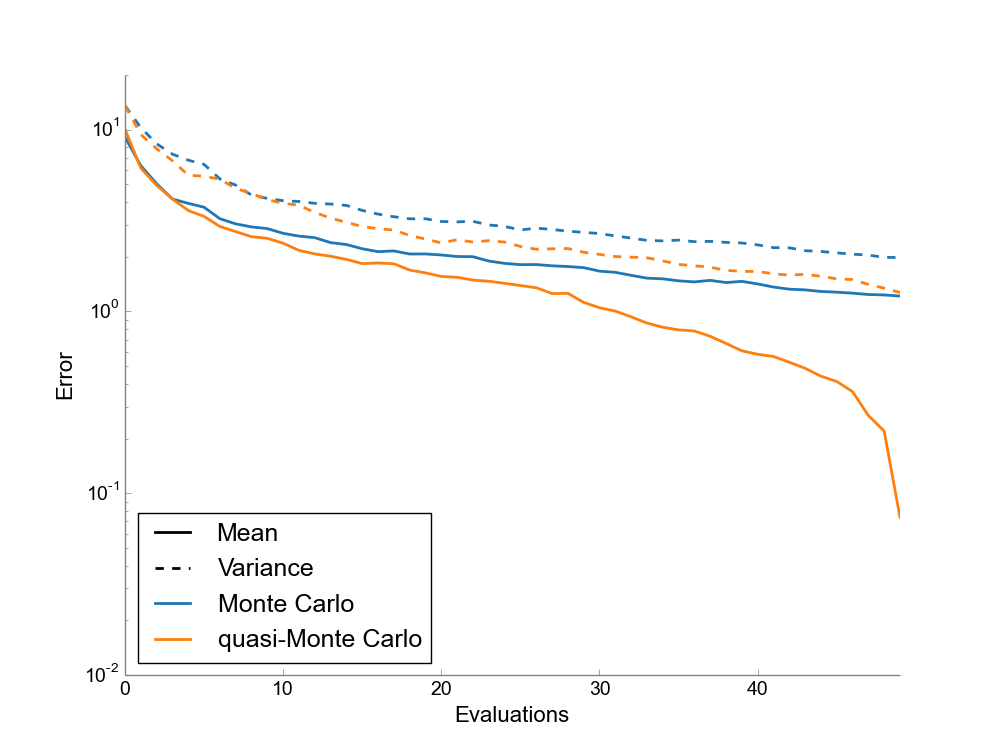
\includegraphics[width=1\textwidth]{qMC-MC_convergence_2D.png}
  \end{center}
\end{frame}



 \begin{frame}
 \frametitle{All random variables can with aid of the Rosenblatt transformations be transformed to/from the uniform distribution}
 \begin{figure}
 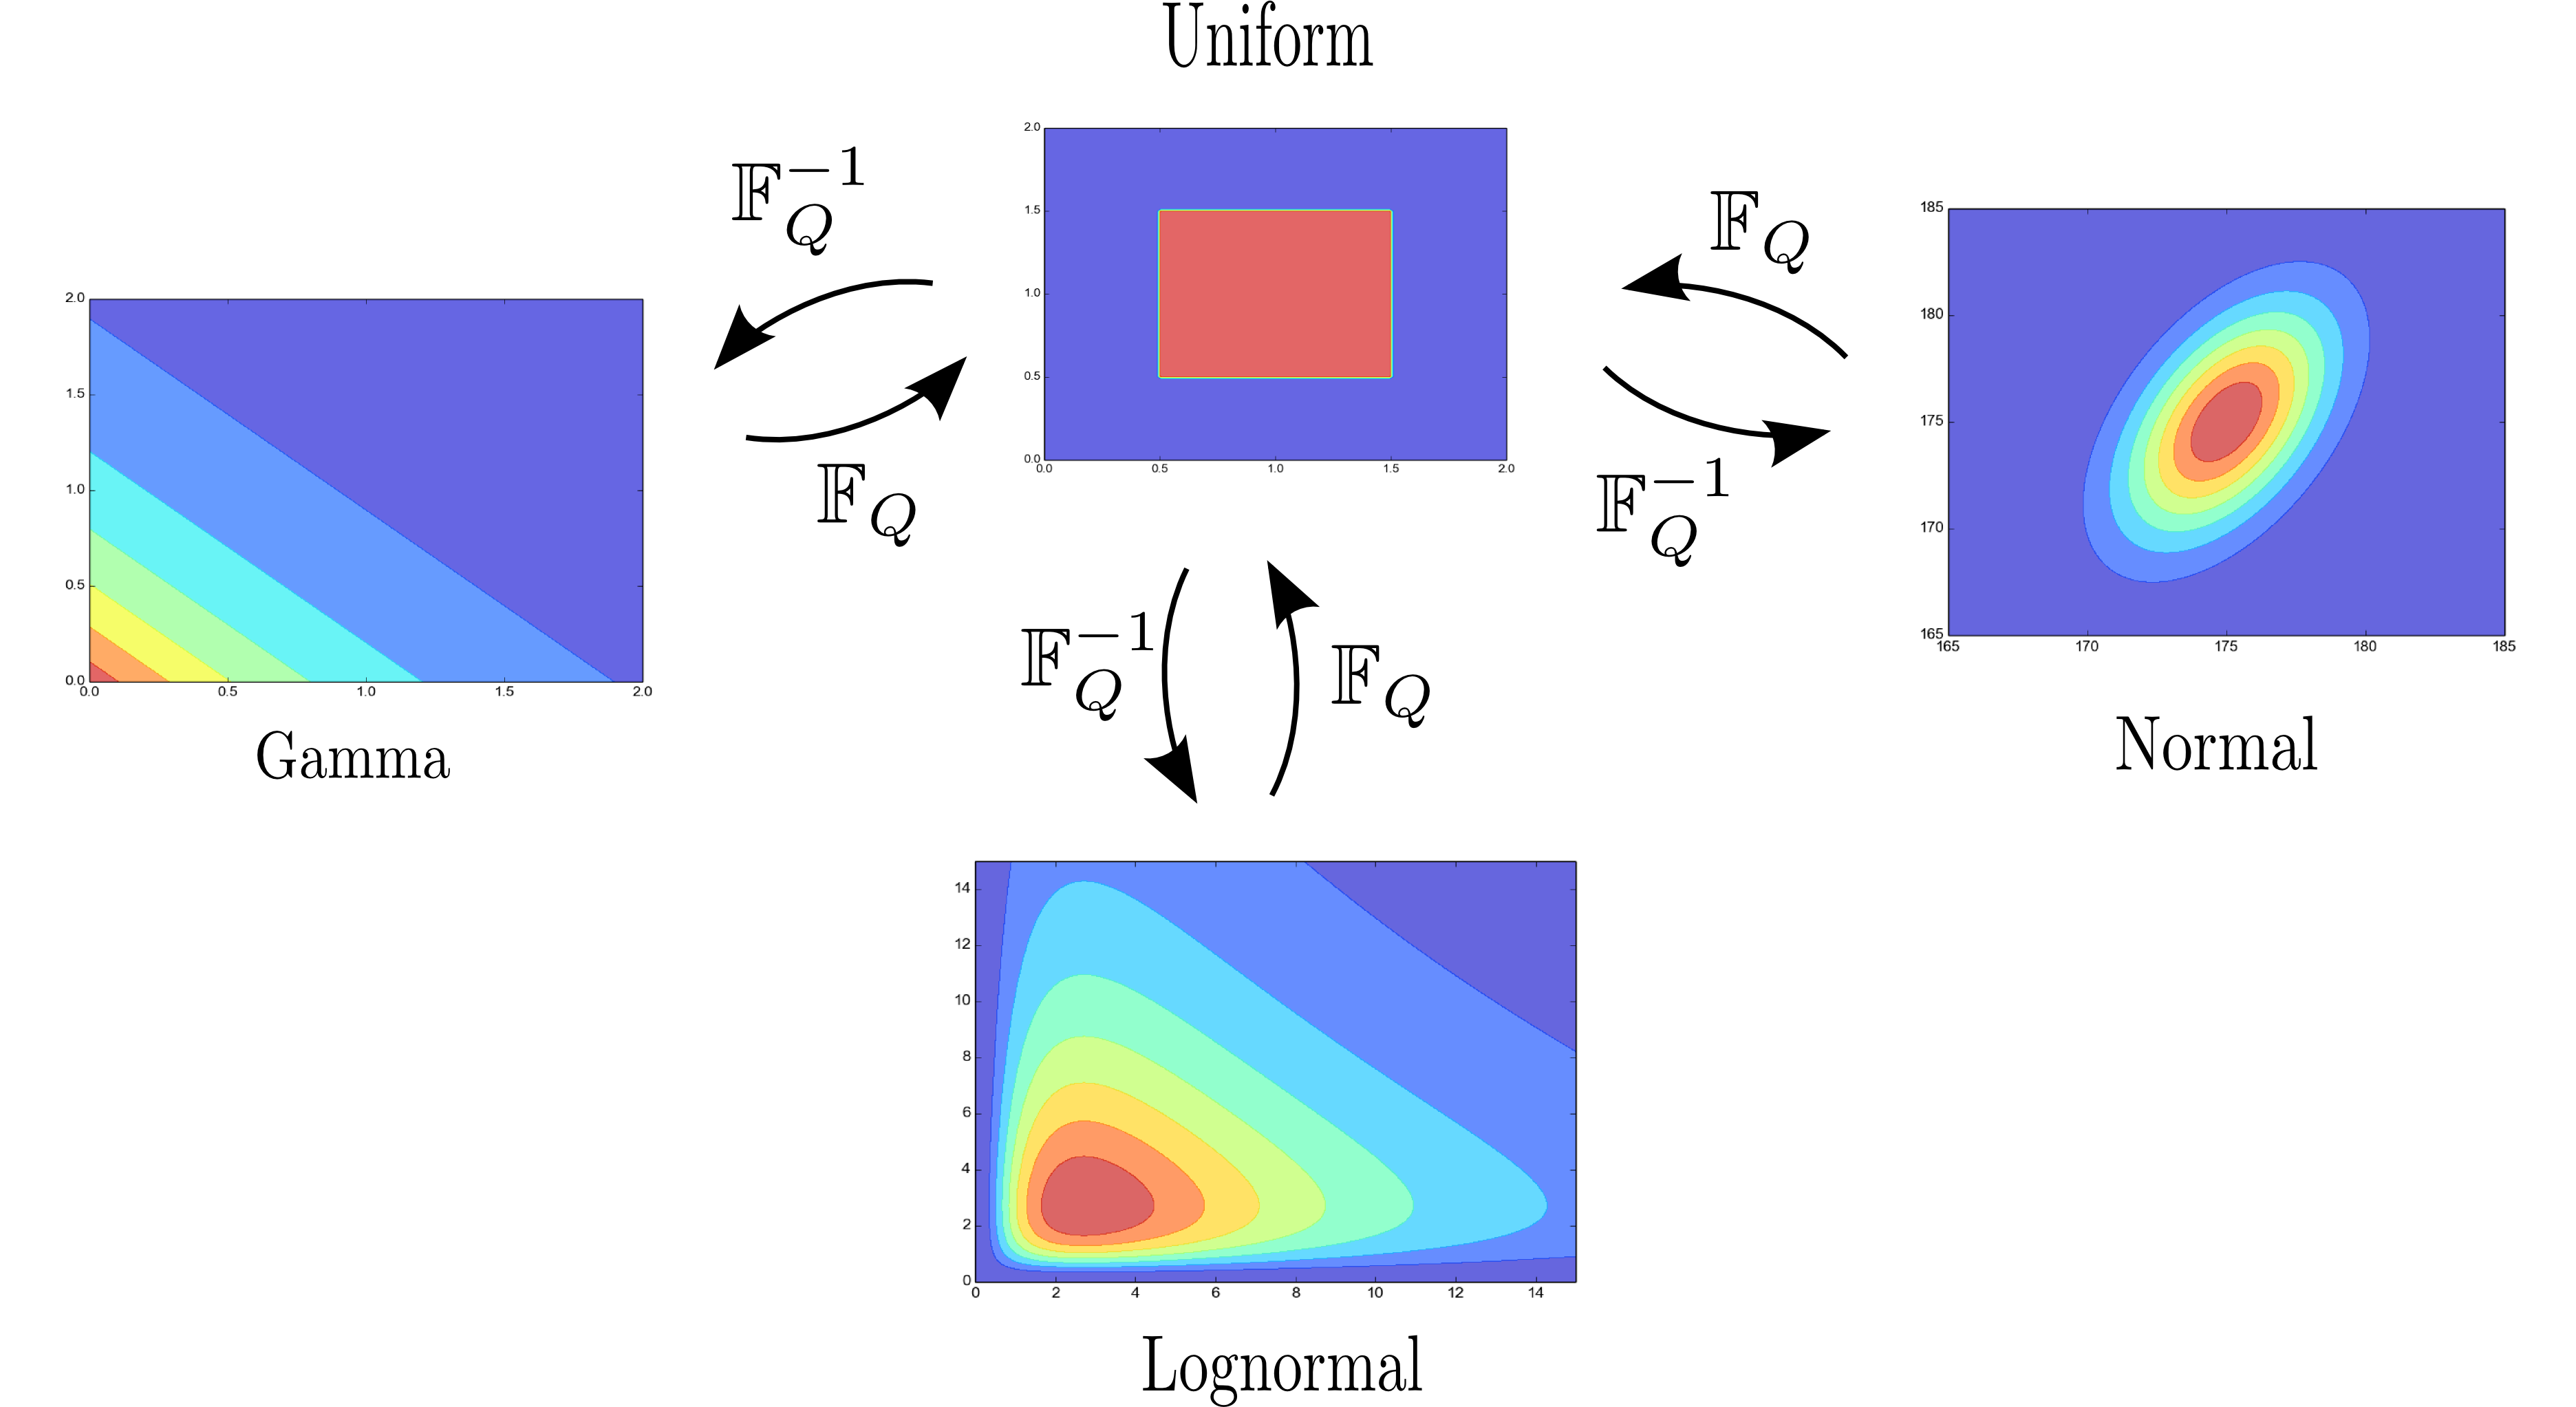
\includegraphics[width = \textwidth]{distributions.png}
 \end{figure}

 \end{frame}

 \begin{frame}
 \frametitle{Chaospy is built around the Rosenblatt transformation which enables several usefull properties}

\begin{itemize}[<+->]
\item Sampling of all probability distributions
\vspace{3mm}
\item Quasi-Monte Carlo sampling is available for any probability distribution
% \vspace{3mm}
% \item Polynomial Chaos expansions are available for any probability distribution, even dependent variables
\end{itemize}

 \end{frame}


% \begin{frame}[fragile]{Using Lagrange polynomials to approximate $u(q)$ ($N$-th degree polynomial interpolation)}{}
%     \begin{align*}
%         u(x;a) &\approx \hat u_M(x;a) =
%         \sum_{n=0}^N c_n(x) P_n(a) & N&=M+1,
%     \end{align*}
%     where
%     \begin{itemize}
%         \item[$c_n$] are model evaluations $u(x, a_n)$
%         \item[$P_n$] are Lagrange polynomials:
%             \begin{align*}
%                 P_n(a) &= \prod_{\substack{m=0 \\ m\neq n}}^N \frac{a-a_n}{a_m-a_n}
%             \end{align*}
%         \item[$a_n$] are collocation nodes
%     \end{itemize}
% \end{frame}


\begin{frame}
  \frametitle{The idea behind Polynomial Chaos (PC) theory is to approximate our model with a polynomial}
  \begin{align*}
      u(x; q) & &\approx && \hat u_M(x;q) && =
      && \sum_{n=0}^N && {\color<3>{red}c_n(x)}\quad && {\color<4>{red}P_n(q)}\\
      &&  &&  &&  &&  && {\color<3>{red}\text{Coefficient}} && {\color<4>{red}\text{Polynomial}}
  \end{align*}

\hspace{10.5mm} $q$ are the uncertain variables
  \begin{align*}
      N = \frac{(M + D)!}{M!D!} - 1, \quad D\text{ is the number of dimensions}\\
  \end{align*}
\pause
Mean and variance are calculated from $\hat u_M(x;q)$
\end{frame}

% \begin{frame}
%   \frametitle{The idea behind Polynomial Chaos (PC) theory is to approximate our model with a polynomial orthogonal in probability space}
%   \begin{align*}
%       u(x; q) \approx \hat u_M(x;q)  &= \sum_{n=0}^N && {\color<3>{red}c_n(x)}\quad && {\color<4>{red}P_n(q)}, \qquad N = \frac{(M + D)!}{M!D!} - 1,\\
%                                      &               && {\color<3>{red}\text{Coefficient}} && {\color<4>{red}\text{Polynomial}}
%   \end{align*}
%
%
% \begin{description}
%     \item[D] - the number of dimensions
%     \item[$q$] - the uncertain variables
% \end{description}
% \end{frame}


\begin{frame}
  \frametitle{}

We have the variance criteria

\[ \Var{|u - \hat u_M|}\]

and want to choose the Best Linear Unbiased Estimator (BLUE)
\begin{align*}
    \E{\hat u_M} &= u\\
    \Var{|u - \hat u_M|} &\leq \Var{|u - \hat u^*|} &    &\forall  u^* \in P_M\\
    &&& \forall M \in N
\end{align*}
    All polynomials $P_n$ and coeffisients $c_n$ are free
\end{frame}



\begin{frame}
    \frametitle{The only numerically stable method for calculating orthogonal polynomials is through the three-term discretized Stiltjes recursion}
    Choosing the Best Linear Unbiased Estimator leads to:
\begin{align*}
\E{P_nP_m} &= 0  & \forall n \neq m\\
\end{align*}

Which is fulfilled by choosing orthogonal polynomials.
\end{frame}


% \begin{frame}
%     \frametitle{The mean and variance now have a simple form}
%     \begin{align*}
%           \E{\hat u_M}&=c_0
%           &
%           \Var{\hat u_M}&=\sum_{n=1}^N c_n^2\E{P_n^2}
%       \end{align*}
% \end{frame}

% \begin{frame}{The mean and variance now have a simple form}{}
%     \begin{alert}{Assumption:}
%         $P_0 = 1$
%     \end{alert}
%     \begin{align*}
%         \onslide<3->{\E{\hat u_M} &=
%         \E{\sum_{n=0}^N c_n P_n}}
%         &
%         \onslide<7->{\Var{\hat u_M} &=
%         \Var{\sum_{n=0}^N c_n P_n}}
%         \\
%         \onslide<4->{&=
%         \sum_{n=0}^N c_n \E{P_n}}
%         &
%         \onslide<8->{&=
%         \sum_{\substack{n=0\\m=0}}^N c_n c_m
%         \left(\E{\!P_nP_m\!}\!-\!\E{\!P_n\!}\!\E{\!P_m\!}\right)}
%         \\
%         \onslide<5->{&=
%         \sum_{n=0}^N c_n \inner{P_n, P_0}}
%         &
%         \onslide<9->{&=
%         \sum_{\substack{n=1\\m=1}}^N c_nc_m\inner{P_n,P_m}-c_0^2}
%         \\
%         \onslide<6->{\E{\hat u_M}&=c_0}
%         &
%         \onslide<10->{\Var{\hat u_M}&=
%         \sum_{n=1}^N c_n^2\norm{P_n}}
%     \end{align*}
% \end{frame}


%
% \begin{frame}
%  \frametitle{The computational essence of Polynomial Chaos}
% \[\hat u_M(x;q) = \sum_{n=0}^N c_n(x) P_n(q)\]
% \vspace{10mm}
%
%  We need to find the orthogonal polynomials $P_n(q)$ and the coefficients $c_n(x)$.
%
% \end{frame}



% \begin{frame}
%  {The only numerically stable method for
%  calculating orthogonal polynomials is through the three-term discretized
%  Stiltjes recursion}
%  \pause
%  Three terms recursion relation:
%  \begin{align*}
%      P_{n+1} &= (x-A_n) P_n - B_n P_{n-1} &
%      P_{-1} &= 0 & P_0 &= 1,
%  \end{align*}
%     \pause
%    where
%    \begin{align*}
%    A_n &= \frac{\langle qP_n,P_n\rangle_Q}{\norm{P_n}^2}
%    &
%   B_n &=
%   \begin{cases}
%   \frac{\norm{P_n}^2}{\norm{P_{n-1}}^2} & n > 0\\
%   \norm{P_n}^2 & n = 0
%   \end{cases}
%    \end{align*}
%   \end{frame}



\begin{chaospy}{The only numerically stable method for calculating orthogonal polynomials is through the three-term discretized Stiltjes recursion}
\begin{lstlisting}[language=python]
dist = cp.Normal()
P = cp.orth_ttr(3, dist)

print P
[1.0, q0, q0^2-1.0, q0^3-3.0q0]
\end{lstlisting}
\end{chaospy}


% \begin{frame}{Least squares minimization leads to a formula for $c_n$, named the \emph{pseudo-spectral method}}
% \vspace{-10mm}
%     \begin{align*}
%         \onslide<1->{ &\min_{c_0,\ldots,c_N} || u- \hat u_M||_Q^2 & \quad\text{where Q is a random vector, i.e. $(a, I )$}\\
%           &\qquad\vdots\quad&\\}
%         \onslide<2>{&c_n = \coef{u}{P_n} & \quad\text{Fourier coefficients}\\}
%         \onslide<3>{&c_n = \int \quad ... \quad dq &\\}
%     \end{align*}
%     The integrals in $c_n$ are approximated by quadrature rules where the probability distribution is used as a weight function.
%
%     % The integrals in $c_n$ are approximated by quadrature rules, which are
%     % optimal if we have a weight function. It turns out that all probability
%     % distribution qualify as weight functions.
% \end{frame}

% \begin{frame}{Coefficients can be calculated using the numerical integration Guassian Quadrature}{}
%     \begin{align*}
%         \onslide<1->{ \min_{c_0,\ldots,c_N} || u- \hat u_M||_Q^2&\\
%           \vdots\qquad&\\}
%         \onslide<2>{c_n = \coef{u}{P_n} & \qquad\text{Fourier coefficients}}
%     \end{align*}
%     where Q is a random vector, i.e. $(a, I )$
%
%     \vspace{5mm}
%
%     Quadrature methods are optimal if we have a weight function, it turns out
%     that all probability distribution qualify as  weight functions.
%
%     The numerical integral approximation is named pseudo-spectral method.
% \end{frame}

%
% \begin{frame}
%  \frametitle{Least squares minimization leads to a formula for $c_n$, named the \emph{pseudo-spectral method}}
%
%  \begin{align*}
%      c_n(x) &= \frac{\inner{ u,P_n}}{\norm{P_n}^2}
%      \onslide<2->{=\frac{\E{uP_n}}{\E{P_n^2}}} \\
%      \onslide<3-> {&=\frac{1}{\E{P_n^2}} \int u(x;q)P_n(q)f_Q(q)dq}
% \onslide<4-> {\approx\\
% \hat{c}_n(x) &= \frac{1}{\E{P_n^2}} \sum_{k=0}^K
% P_n(q_k)u(x;q_k)f(q_k)\omega_k}
% \end{align*}
%
% \onslide<3->
% $q_k$ quadrature nodes, $\omega_k$ quadrature weights
%
% \end{frame}





%
% \begin{frame}
%     This leads to
% \begin{align*}
% \E{P_nP_m} &= 0  & \forall n \neq m\\
% c_n &= \frac{\E{uP_n}}{\E{P_n^2}}
% \end{align*}
%
% Solution:
% \begin{align*}
%     \E{P_nP_m} &= 0 & &\text{Fulfilled by choosing orthogonal polynomials} \\
%     c_n &&& \text{Can be approximated by quadrature rules, }\\
%         &&& \text{the probability distribution is used as a weight function}
% \end{align*}
% \end{frame}




\begin{frame}
\frametitle{$c_n$ is approximated by quadrature rules}
    Choosing the Best Linear Unbiased Estimator leads to:

\begin{align*}
c_n &= \frac{\E{uP_n}}{\E{P_n^2}}
\end{align*}
$c_n$ is approximated by quadrature rules where the probability distribution is used as a weight function.
\end{frame}



\begin{chaospy}{
  Generating nodes and weights in Chaospy}
     % TODO
     % high: add code for 1-D gen_quad
     % high: list quadrature schemes
    \scriptsize
\onslide<1->
\begin{lstlisting}[language=python]
dist = cp.Normal()
nodes, weights = cp.generate_quadrature(2, dist, rule="G")
|\pause|
print nodes
[[-1.73205081  0.          1.73205081]]
print weights
[ 0.16666667  0.66666667  0.16666667]
\end{lstlisting}
\normalsize

\end{chaospy}





\begin{chaospy}{A full implementation with the pseudo-spectral method
    in Chaospy}
    \scriptsize
    % TODO
    % high: make it 2-D problem
%  def u(x, a, I):
%    return I*np.exp(-a*x)
%  |\pause|
 \begin{lstlisting}[language=python]
dist_a = cp.Uniform(0, 0.1)
dist_I = cp.Uniform(8, 10)
dist = cp.J(a,I)
|\pause|
P = cp.orth_ttr(2, dist)
|\pause|
nodes, weights = cp.generate_quadrature(3, dist)
|\pause|
x = np.linspace(0, 10, 100)
samples_u = [u(x, *node) for node in nodes.T]
|\pause|
u_hat = cp.fit_quadrature(P, nodes, weights, samples_u
                          rule="Gaussian")
|\pause|
mean = cp.E(u_hat, dist)
var = cp.Var(u_hat, dist)
\end{lstlisting}
\end{chaospy}


\begin{frame}
 \frametitle{Convergence of our model problem}
 % TODO
 % high: error formulae
%   \begin{align*}
%   \varepsilon_E &= \int_0^{10}|E(u) - E(\hat{u})|\,dx &
%   \varepsilon_{Var} &= \int_0^{10}|Var(u) - Var(\hat{u})|\,dx
%   \end{align*}

\begin{figure}
    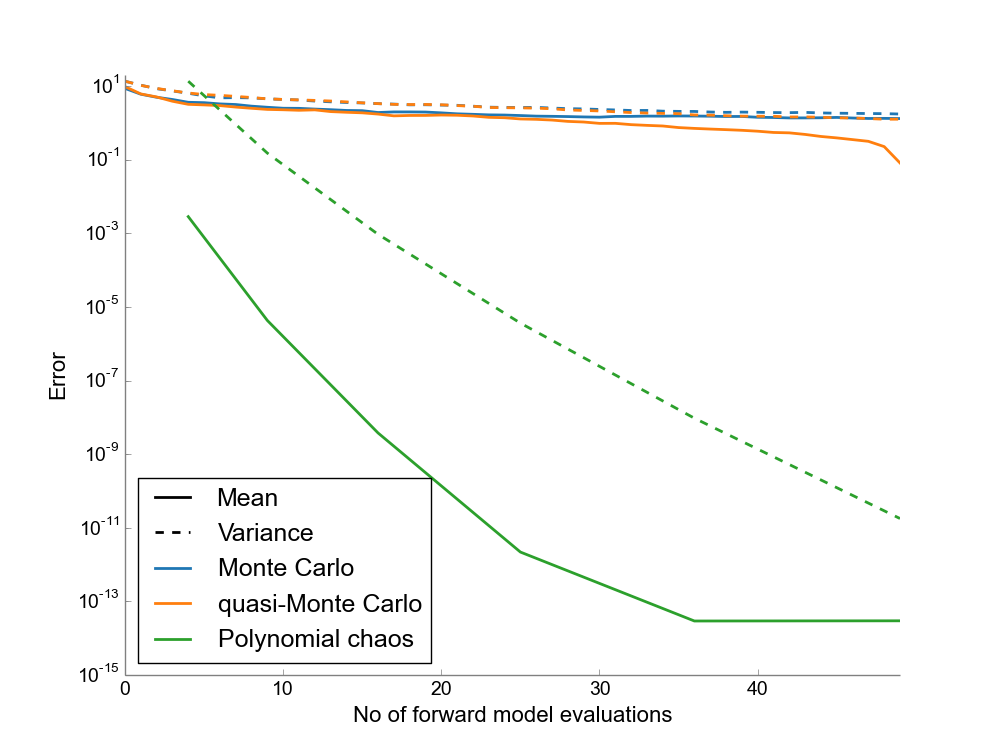
\includegraphics[width=1\textwidth]{qMC-MC-PC_convergence_2D.png}
  \end{figure}

 \end{frame}




 \begin{frame}{Different problems require different quadrature rules}{}
     {
         \def\arraystretch{1.2}
 \begin{tabular}{ll|l}
  Key & & Description\\\hline
     "Gaussian"& "G" &    Optimal Gaussian quadrature.\\
     "Legendre"& "E" &    Gauss-Legendre quadrature\\
     "Clenshaw"& "C" &    Clenshaw-Curtis quadrature.\\
     "Leja"& ``J" &          Leja quadrature.\\
     "Genz"& "Z" &        Hermite Genz-Keizter 16 rule.\\
     "Patterson" & "P"&    Gauss-Patterson quadrature rule.\\
 \end{tabular}
 }
 \end{frame}




%  \begin{frame}
%   \frametitle{The point collocation method is an alternative to the
%   pseudo-spectral method}
%
% \begin{enumerate}[<+->]
% \item Psuedo-spectral method:
% \begin{enumerate}[<+->]
% \item Determine polynomial approximation of model by least squares
% minimization in a space weighted with the probability distribution
% \vspace{1mm}
% \item Approximate integrals in $c_n$ by quadrature rules
% \end{enumerate}
% \vspace{5mm}
% \item Point collocation method:
% \begin{enumerate}[<+->]
% \item Determine polynomial approximation of model by least squares
% minimization in a vector space as in regression (or overdetermined matrix systems)
% \vspace{1mm}
% \item Need to choose a set of nodes (regression points)
% \end{enumerate}
% \end{enumerate}
% \end{frame}
%
%
%
% \begin{chaospy}{Code for point collocation}
%     % TODO
%     % remove "H" and rule="LS" and simulate again again.
%     \scriptsize
%  \begin{lstlisting}[language=python]
% def u(x, a, I):
%   return I*np.exp(-a*x)
%  |\pause|
% dist_a = cp.Uniform(0, 0.1)
% dist_I = cp.Uniform(8, 10)
% dist = cp.J(dist_a, dist_I)
% |\pause|
% x = np.linspace(0, 10, 100)
%  |\pause|
% P = cp.orth_ttr(3, dist)
%  |\pause|
% nodes = dist.sample(2*len(P)) |\pause|
% samples_u = [u(x, *node) for node in nodes.T] |\pause|
%
% u_hat = cp.fit_regression(P, nodes, samples_u)
%  \end{lstlisting}
%
% \end{chaospy}



% \begin{frame}{What is best of pseudo-spectral and point collocation method? It's problem dependent!}{}
%     % TODO
%     % Plot!
%     % SC nested-CC sparsegrid vs. PC with S-rule and LS-fit vs. MC
%       \begin{figure}
%   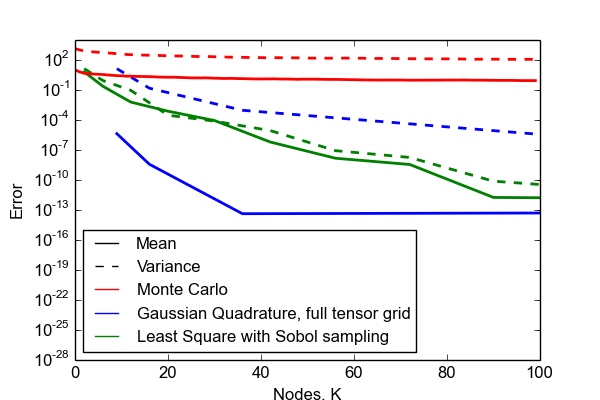
\includegraphics[width=0.85\textwidth]{MC_convergence_2D_diff.png}
%  \end{figure}
% \end{frame}


% \begin{frame}{Which method to choose for your problem depends on the problem}{}
%     \scriptsize
%     \begin{tabular}{r|lll}
%         & \bf Pseudo-spectral &
%         \bf Point collocation & \bf Monte Carlo \\ \\ \hline \pause\\
%         Efficiency              & \color{green} Highest
%             & \color{green} Very high & \color{red} Very low  \pause\\\\
%         Stability               & \color{red} Low
%             & Medium   & \color{green}Very high \pause\\\\
%             Dimension-independence  & \color{red} Lowest
%             & \color{red} Low    & \color{green} Highest
%     \end{tabular}
% \end{frame}


% \begin{chaospy}{A surrogate model allows for computational cheap statistical analysis}
%     \scriptsize
%  \begin{lstlisting}[language=python]
% u_hat, c_hat = cp.fit_quadrature(
%         P, nodes, weights, solves, retall=True)
% |\pause|
% mean =  cp.E(u_hat, dist)
% var = cp.Var(u_hat, dist)
% |\pause|
%
% mean = c_hat[0]
% norms2 = cp.E(P**2, dist)[1:]
% c2 = c_hat[1:]**2
% var = np.sum(c2*norms2)
% |\pause|
%
% samples_q = dist.sample(10**6)
% samples_u = u_hat(*samples_q)
% mean = np.mean(samples_u,1)
% var = np.var(samples_u,1)
% \end{lstlisting}
% \end{chaospy}


 \begin{frame}
 \frametitle{Chaospy handles Polynomial Chaos expansions with stochastically dependent variables}

Dependent variables break the orthogonality properties of the polynomials.

\pause

\vspace{7mm}

The Rosenblatt transformation can be used to model dependent
variables effectively as a parameterization of
independent variables
\begin{align*}
        \hat u_M(x; q)
        \onslide<2->{= \hat u_M(x; T(r))}
        \onslide<3->{= \sum_{n=0}^N c_n(x) P_n(r)}
    \end{align*}

 \end{frame}


\begin{chaospy}{The polynomial approximation can be used as a surrogate model, which allows for computational cheap statistical analysis}
    \scriptsize
 \begin{lstlisting}[language=python]
u_hat = cp.fit_quadrature(P, nodes, weights, solves)
|\pause|
samples_q = dist.sample(10**6)
samples_u = u_hat(*samples_q)
|\pause|
mean = np.mean(samples_u, 1)
var = np.var(samples_u, 1)
\end{lstlisting}
\end{chaospy}


\begin{frame}{Advantages and disadvantages of Chaospy}{}
\onslide<1->\bf \color{green} {Advantages}
\begin{itemize}
\onslide<1->\gooditem Modular
\onslide<3->\gooditem The programming syntax lies close to the mathematical theory
\onslide<5->\gooditem Supports both Monte Carlo and Polynomial Chaos
\onslide<6->\gooditem Handles dependent variables
\end{itemize}
\vspace{8mm}
\onslide<1->\bf\color{red} Disadvantages
\begin{itemize}
\onslide<2->\baditem Modular
\onslide<4->\baditem The programming syntax lies close to the mathematical theory
\onslide<7->\baditem Slow
\end{itemize}

\end{frame}





% \begin{frame}
%  \frametitle{Some random variables are dependent}
%  \begin{figure}
%  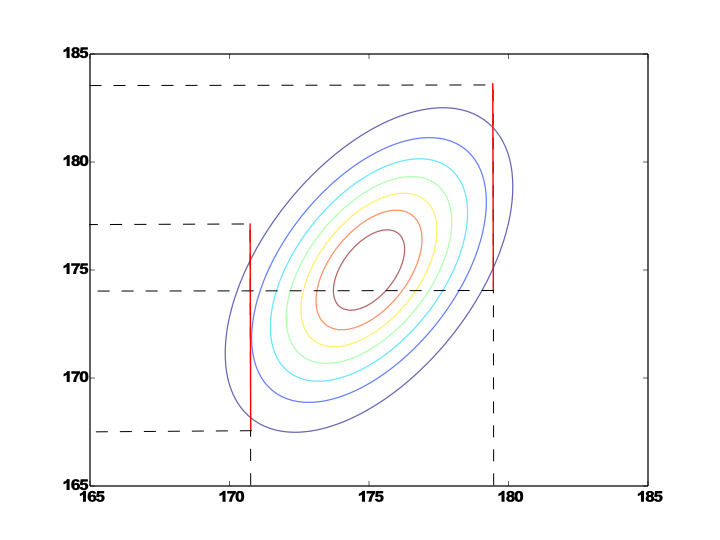
\includegraphics[width = 0.9\textwidth]{dependent.png}
%  \end{figure}
%
%  \end{frame}


%
% \begin{frame}{Transformations manipulates probability distributions}
% \begin{figure}
%  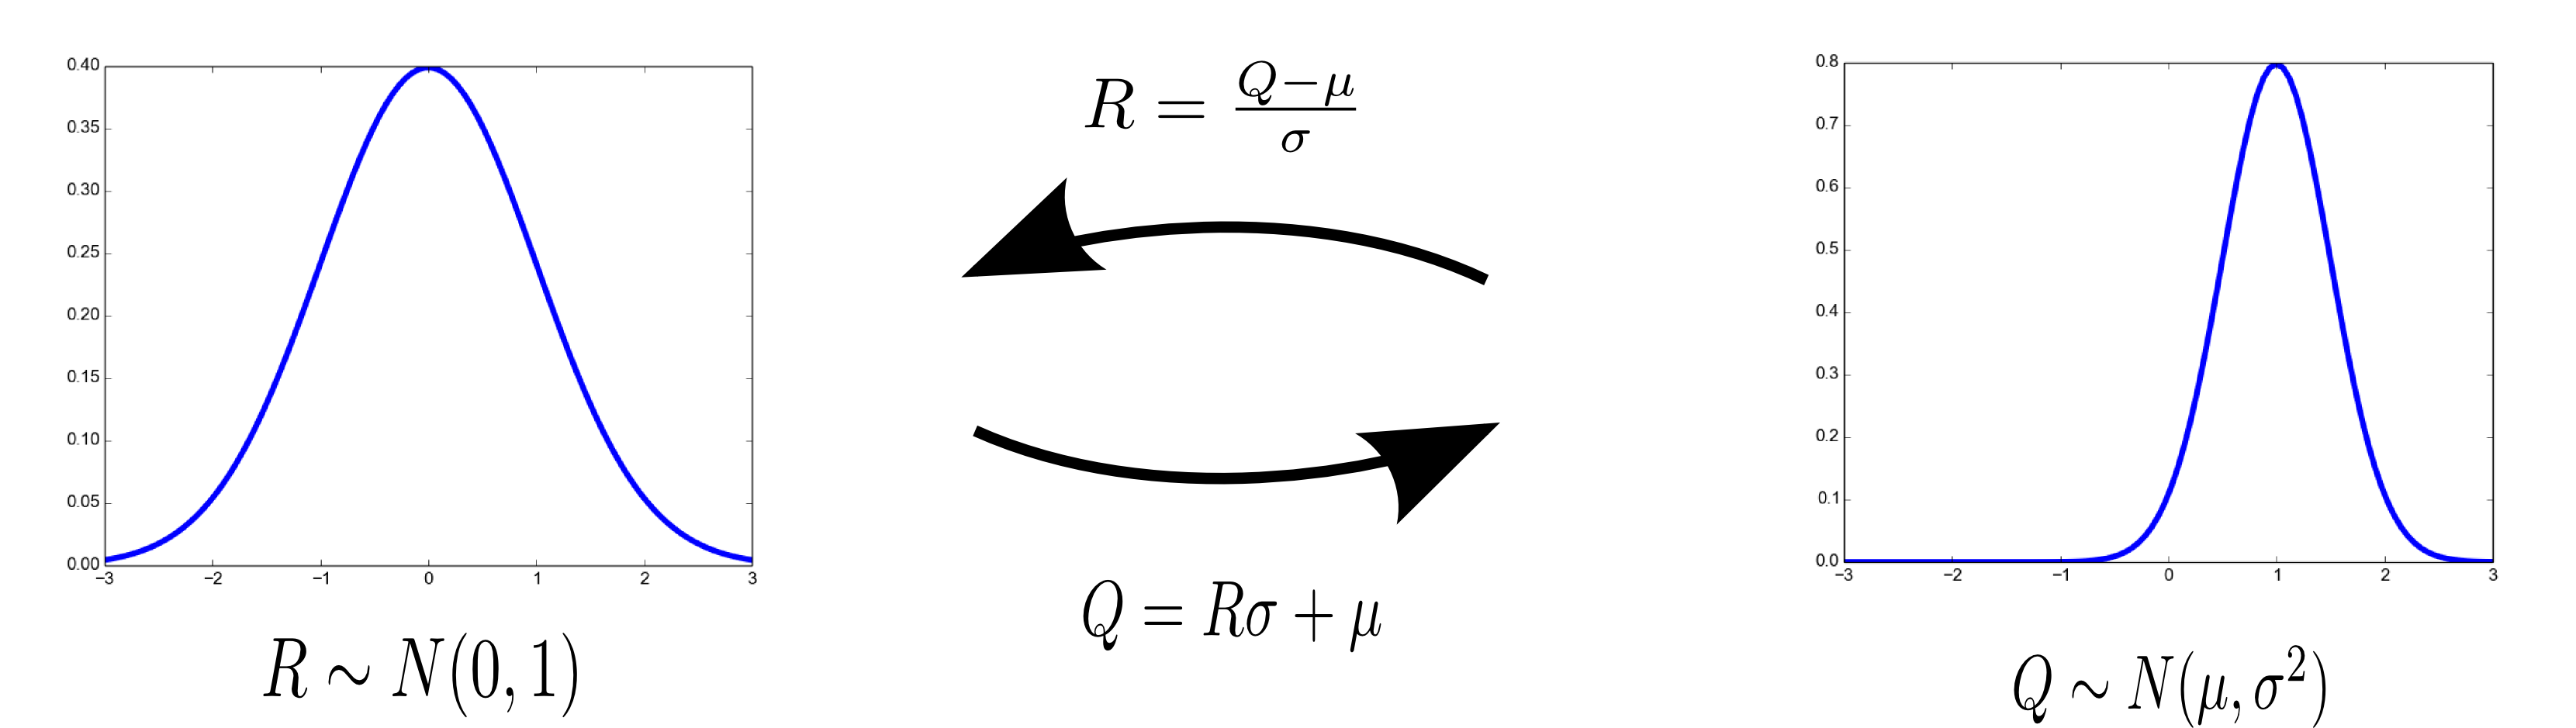
\includegraphics[width=\textwidth]{trans2.png}
% \end{figure}
% \end{frame}




%
% \begin{frame}
%  \frametitle{Dependent variables break the orthogonality property of Polynomal Chaos!}
%  \scriptsize
%  \[  P_{\mathfrak i} = P_{i_1}^{(1)}P_{i_2}^{(2)}\cdots P_{i_D}^{(D)} \qquad \mathfrak i = (i_1,i_2,...,i_D)\]
%  \pause
%  \begin{align*}
%      \inner{ P_\mathfrak{i},P_\mathfrak{j}} &= E(P_\mathfrak{i},P_\mathfrak{j})\\
%   \onslide<3-> {&=\E{P_{i_1}^{(1)}\cdots P_{i_D}^{(D)}P_{j_1}^{(1)}\cdots P_{j_D}^{(D)}}}\\
%   \onslide<4-> {&=\E{P_{i_1}^{(1)}P_{j_1}^{(1)}}\cdots \E{P_{i_D}^{(D)}P_{j_D}^{(D)}}}\\
%   \onslide<5-> {&=\dots}\\
%   \onslide<5-> {&=\norm{P_{\mathfrak{i}}^{(1)}}\delta_{\mathfrak{i}\mathfrak{j}}}
%  \end{align*}
%  \onslide<6->
% \begin{alert}{But the problem is:}
% \[\E{uv} \neq \E{u}\E{v} \qquad \text{when $u$ and $v$ are
% stochastically dependent}\]
%  \end{alert}
%  \end{frame}






%  \begin{chaospy}{Point collocation with Rosenblatt transformation}
%  \scriptsize
%  \begin{lstlisting}[language=Python]
% def u(x,a, I):
%     return I*np.exp(-a*x)
% |\pause|
% dist_R = cp.J(cp.Normal(), cp.Normal())
% C = [[1, 0.5], [0.5, 1]]
% mu = [0, 0]
% dist_Q = cp.MvNormal(mu, C)
% |\pause|
% P = cp.orth_ttr(M, dist_R)|\pause|
% nodes_R = dist_R.sample(2*len(P), "M")|\pause|
% nodes_Q = dist_Q.inv(dist_R.fwd(nodes_R))
% |\pause|
% x = np.linspace(0, 1, 100)
% samples_u = [u(x, *node) for node in nodes_Q.T]|\pause|
% u_hat = cp.fit_regression(P, nodes_R, samples_u)
% \end{lstlisting}
% \end{chaospy}
%
%
%
%  \begin{chaospy}{Pseudo-spectral with Rosenblatt transformation}
%  \scriptsize
%  \begin{lstlisting}[language=Python]
% def u(x,a, I):
%     return I*np.exp(-a*x)
% |\pause|
% C = [[1,0.5],[0.5,1]]
% mu = np.array([0, 0])
% dist_R = cp.J(cp.Normal(), cp.Normal())
% dist_Q = cp.MvNormal(mu, C)
%
% P = cp.orth_ttr(M, dist_R)
% nodes_R, weights_R = cp.generate_quadrature(M+1, dist_R)|\pause|
% nodes_Q = dist_Q.inv(dist_R.fwd(nodes_R))|\pause|
% weights_Q = weights_R*\
%     dist_Q.pdf(nodes_Q)/dist_R.pdf(nodes_R)
% |\pause|
% x = np.linspace(0, 1, 100)
% samples_u = [u(x, *node) for node in nodes_Q.T]|\pause|
% u_hat = cp.fit_quadrature(P, nodes_R, weights_Q, samples_u)
% \end{lstlisting}
% \end{chaospy}



\begin{frame}{Summary: Chaospy is a modular software for uncertainty quantification with syntax that lies close to the mathematical theory}

\begin{tikzpicture}[remember picture, overlay, font=\sffamily]
    \node [align=left, xshift=0.3\textwidth,yshift=0.1\textwidth] (image1) at (current page.center)
          {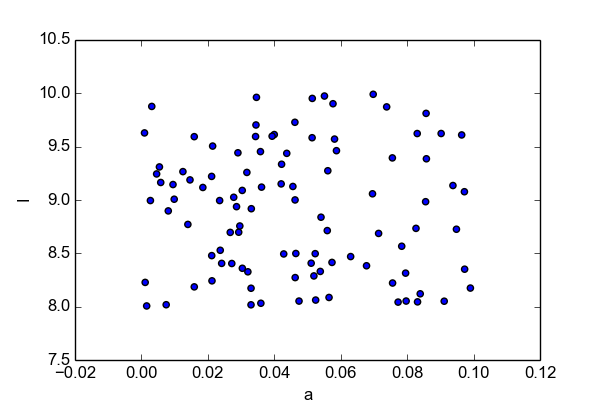
\includegraphics[width = 0.3\textwidth]{samples.png}};
    \node[align=left] at (image1.west) {\hspace{-7cm} \bf Advanced Monte Carlo methods};
  \end{tikzpicture}


\begin{tikzpicture}[remember picture, overlay, font=\sffamily]
    \node [align=left, xshift=0.3\textwidth,yshift=-0.15\textwidth] (image2) at (current page.center)
          {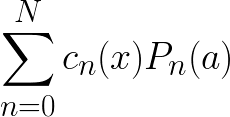
\includegraphics[width = 0.25\textwidth]{pc.png}};
    \node[align=left] at (image2.west) {\hspace{-7.95cm} \bf Polynomial Chaos expansions};
  \end{tikzpicture}



  \begin{tikzpicture}[remember picture, overlay, font=\sffamily]
      \node [align=left, xshift=0.49\textwidth,yshift=-0.37\textwidth] (image2) at (current page.center)
            {
\includegraphics[width = 0.35\textwidth]{cinpla.png}};
    \end{tikzpicture}

    \begin{tikzpicture}[remember picture, overlay, font=\sffamily]
        \node [align=left, xshift=-0.45\textwidth,yshift=-0.37\textwidth] (image2) at (current page.center)
              {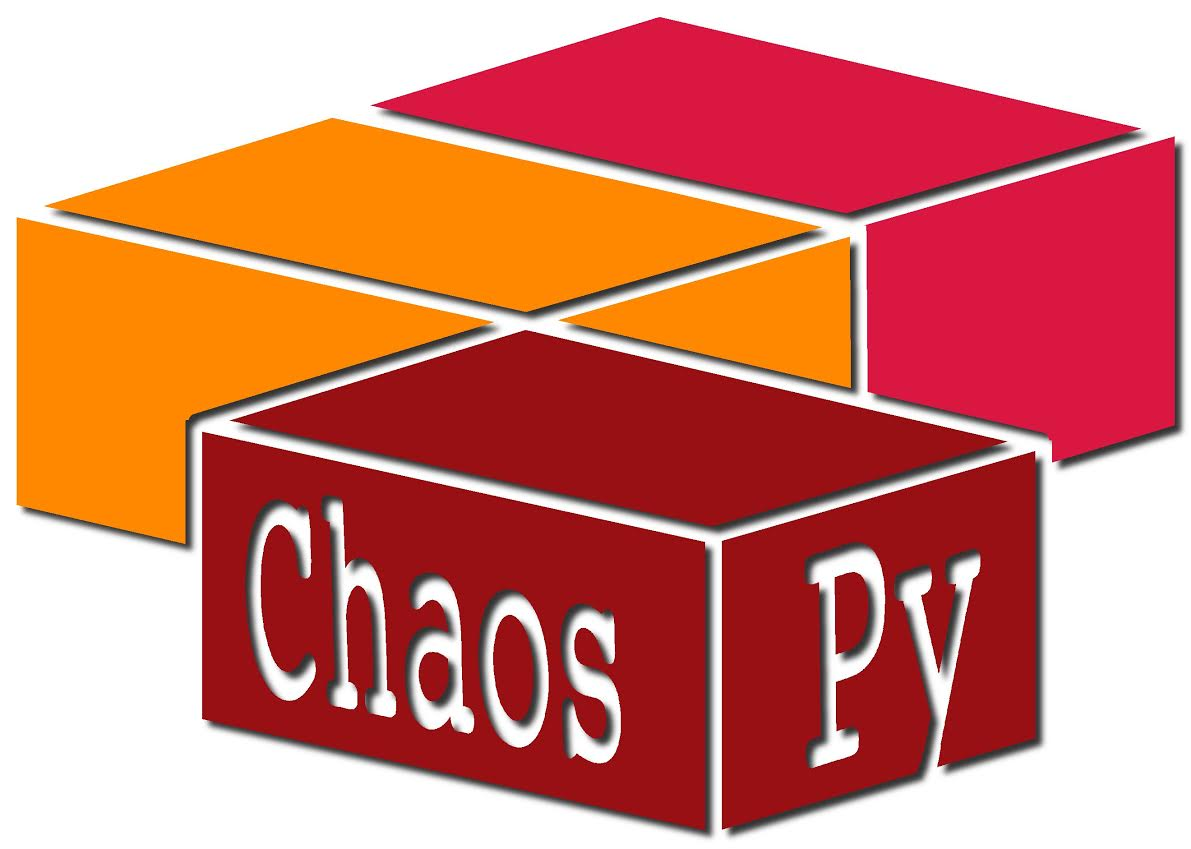
\includegraphics[width = 0.18\textwidth]{chaospy_logo.jpg}};
      \end{tikzpicture}

% \pause
% \begin{tikzpicture}[remember picture, overlay, font=\sffamily]
%
%   \node[align=left, yshift=0.1\textwidth] at (current page.south){ \bf Questions?};
% \end{tikzpicture}
%
% \vspace{3.5cm}
%
%   \begin{alert}{Installation instructions:}\\
%   \scriptsize
%       \href{https://github.com/hplgit/chaospy}{https://github.com/hplgit/chaospy}\\
% %\verb;http://github.com/hplgit/chaospy/;
%   \end{alert}
%
%
%
%   \begin{alert}{References:}\\
%   \scriptsize
%       Feinberg, J., \& Langtangen, H. (2015). Chaospy: An open source tool for designing methods of uncertainty quantification. Journal Of Computational Science, 11, 46-57\\
%       \href{http://www.sciencedirect.com/science/article/pii/S1877750315300119}{http://www.sciencedirect.com/science/article/pii/S1877750315300119}
%   \end{alert}

\end{frame}


\begin{frame}{Summary: Chaospy is a modular software for uncertainty quantification with syntax that lies close to the mathematical theory}

  \begin{alert}{Installation instructions:}\\
  \scriptsize
      \href{https://github.com/hplgit/chaospy}{https://github.com/hplgit/chaospy}\\
%\verb;http://github.com/hplgit/chaospy/;
  \end{alert}


\vspace{7mm}

  \begin{alert}{References:}\\
  \scriptsize
      Feinberg, J., \& Langtangen, H. (2015). Chaospy: An open source tool for designing methods of uncertainty quantification. Journal Of Computational Science, 11, 46-57\\
      \href{http://www.sciencedirect.com/science/article/pii/S1877750315300119}{http://www.sciencedirect.com/science/article/pii/S1877750315300119}
  \end{alert}

  \begin{tikzpicture}[remember picture, overlay, font=\sffamily]
      \node [align=left, xshift=0.49\textwidth,yshift=-0.37\textwidth] (image2) at (current page.center)
            {
\includegraphics[width = 0.35\textwidth]{cinpla.png}};
    \end{tikzpicture}

    \begin{tikzpicture}[remember picture, overlay, font=\sffamily]
        \node [align=left, xshift=-0.45\textwidth,yshift=-0.37\textwidth] (image2) at (current page.center)
              {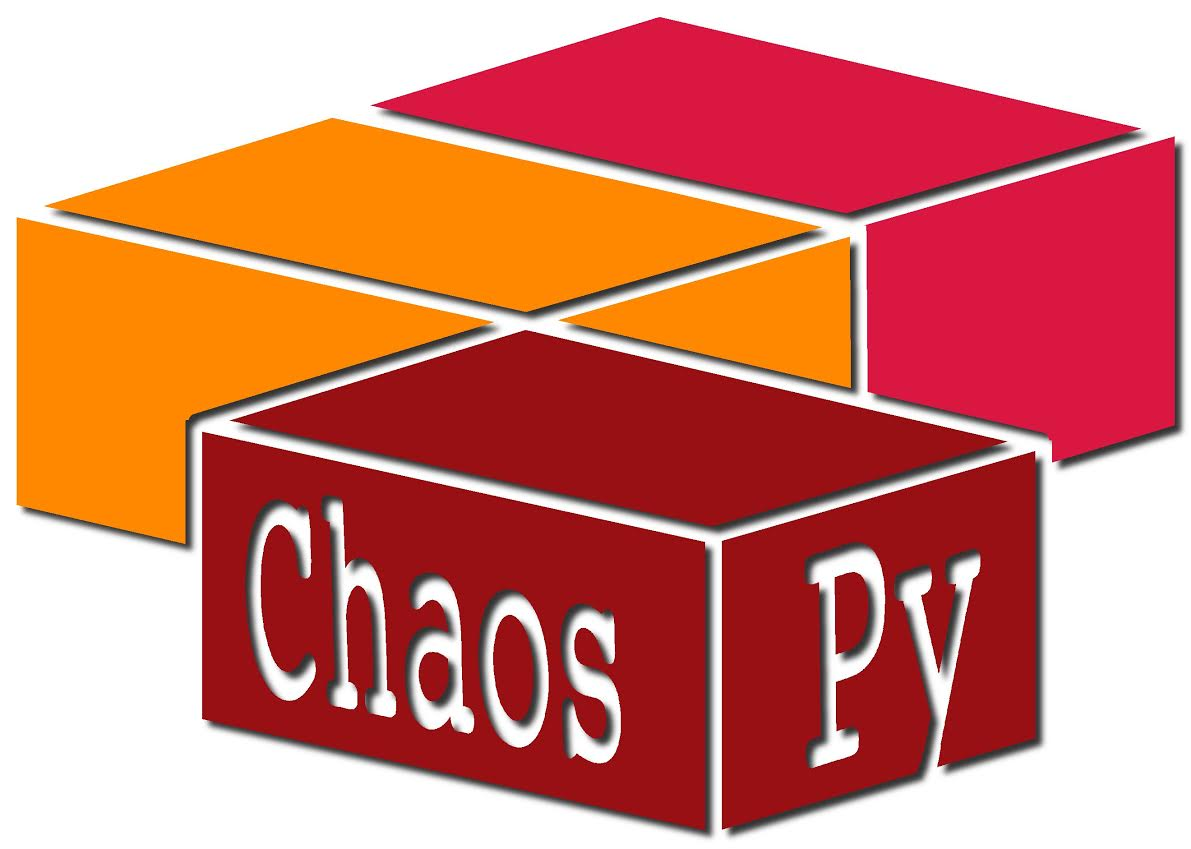
\includegraphics[width = 0.18\textwidth]{chaospy_logo.jpg}};
      \end{tikzpicture}


\begin{tikzpicture}[remember picture, overlay, font=\sffamily]

  \node[align=left, yshift=0.15\textwidth] at (current page.south){ \bf \large Questions?};
\end{tikzpicture}



\end{frame}


\end{document}
